\documentclass[
    aps,
    prd,
    reprint,
    amsmath,
    amssymb,
    nofootinbib,
    superscriptaddress
]{revtex4-2}


\usepackage[utf8]{inputenc}
\usepackage[T1]{fontenc}
\usepackage{graphicx}
\usepackage{booktabs}
\usepackage{amsmath}
\usepackage{amssymb}
\usepackage{bm}
\usepackage{hyperref}
\usepackage[table]{xcolor}
\usepackage{float}
\usepackage{siunitx}
\usepackage{multirow}
\usepackage{enumitem}
\usepackage{placeins}
\usepackage{tikz}
\usepackage{listofitems} % for \readlist to create arrays

\tikzstyle{mynode}=[thick,draw=blue,fill=blue!20,circle,minimum size=22]

\usepackage{amsmath} % for aligned
\usepackage{listofitems} % for \readlist to create arrays
\usetikzlibrary{arrows.meta} % for arrow size
\usepackage[outline]{contour} % glow around text
\contourlength{1.4pt}

% COLORS
\usepackage{xcolor}
\colorlet{myred}{red!80!black}
\colorlet{myblue}{blue!80!black}
\colorlet{mygreen}{green!60!black}
\colorlet{myorange}{orange!70!red!60!black}
\colorlet{mydarkred}{red!30!black}
\colorlet{mydarkblue}{blue!40!black}
\colorlet{mydarkgreen}{green!30!black}

% STYLES
\tikzset{
  >=latex, % for default LaTeX arrow head
  node/.style={thick,circle,draw=myblue,minimum size=22,inner sep=0.5,outer sep=0.6},
  node in/.style={node,green!20!black,draw=mygreen!30!black,fill=mygreen!25},
  node hidden/.style={node,blue!20!black,draw=myblue!30!black,fill=myblue!20},
  node convol/.style={node,orange!20!black,draw=myorange!30!black,fill=myorange!20},
  node out/.style={node,red!20!black,draw=myred!30!black,fill=myred!20},
  connect/.style={thick,mydarkblue}, %,line cap=round
  connect arrow/.style={-{Latex[length=4,width=3.5]},thick,mydarkblue,shorten <=0.5,shorten >=1},
  node 1/.style={node in}, % node styles, numbered for easy mapping with \nstyle
  node 2/.style={node hidden},
  node 3/.style={node out}
}
\def\nstyle{int(\lay<\Nnodlen?min(2,\lay):3)} % map layer number onto 1, 2, or 3


\newcommand{\grayrule}{%
    \arrayrulecolor{gray!45}
    \specialrule{0.3pt}{3pt}{3pt}
    \arrayrulecolor{black}
}


\hypersetup{
    colorlinks=true,
    linkcolor=blue,
    citecolor=blue,
    urlcolor=blue
}

\newcolumntype{P}[1]{>{\begin{minipage}[t]{#1}\raggedright\arraybackslash}l<{\end{minipage}}}



\begin{document}

\title{Project 3, FYS-STK3155\\
Pricing European Options with Physics-Informed Neural Networks: Solving the Black-Scholes Equation via the Heat Equation}

\author{Albert Sjåvåg}
\author{Teodor Aursnes}
\author{Jørgen S. Florholmen}
\affiliation{University of Oslo, Department of Physics}

\date{\today}


\begin{abstract}
In this project we are looking at the Black & Scholes PDE for european call option. We will present it and solve i analytically through the heat equation and we will later on experiment with two different types of neural networks... blablabla


\end{abstract}

\maketitle

\section{{Introduction}}
%Often referred to as "the trillion dollar equation", the Black-Scholes-Merton model 

\section{Theory \& methods}\label{sec:theory}
    %As you now know, the Black-Scholes equation is closely related to the heat equation in physics. In fact, we can, and we will, solve the Black-Scholes PDE using the heat equation and its solution. Before doing so, we need to familiarize ourself with the Black-Scholes model, which describes the world in which we will be working in throughout this report. 
 
\subsection{The Black-Scholes model}

First of all, we need to establish which assumptions which are made for the Black-Scholes model. Remember that the Black-Scholes equation is used to price options or other financial derivatives on some underlying, often stocks. The first assumption of the model is that the price of the underlying itself follows a geometric Brownian motion (GBM) with drift $\mu$ and volatility $\sigma$. For simplification, we will also assume that our underlying (which we will call a  "stock") pays no dividends over the interval of time under consideration. The process for the stock price is described by the following equation:
\begin{equation*}
    dS_t = \mu S_tdt~+~\sigma S_tdW_t
\end{equation*}
where $\mu$ and $\sigma$ are constant. 
Further, we assume that there exists a money market account (MMA), where we can borrow and lend money at a constant risk free rate $r$. Unless otherwise specified, we assume that $r>0$. If you put $B_0$ in the MMA at time $0$, at time $t$, you end up with
\begin{equation*}
    B_t = e^{rt}B_0,
\end{equation*}
where, over any discrete interval of time, r is the continuously compounded risk free rate. Finally, we assume that trading takes places continuously, and that there are no transaction costs, no indivisibility, no short-sales constraints and no taxes on financial gains. 

\subsection{Stochastic calculus \& the BS equation}
Now that we know under which rules we are playing, we can try to find an equation that gives us the price of the derivative at time t. Consider a derivative which, at time T, pays off an amount $g(S_T)$ depending on $S_T$. For example, consider a European call option which gives you the right, but not the obligation, to buy a stock for the price K at expiry T. Then $g(S_T) = max\{S_T-K, 0\}$. 

Now, let $f_t$ be the price of the derivative at time $t$. The question is, given $S_t, \mu, \sigma, r, T$ and a payoff function $g(\cdot)$, what should the price $f_t$ be? Can we write it as a function $V(S_t,t)$? The Black-Scholes equation is the answers to this exact question, and we will see how we can derive it, but first we need to introduce some notions from stochastic calculus, which are essential to the derivation. 

\subsubsection{Stochastic calculus}
To focus on the more relevant parts of this project we will keep this section short, only containing the core essentials. First, let $X$ be(?) a stochastic process, more specifically a geometric Brownian motion, and let its random evolution be governed by $dX_t = \mu X_tdt + \sigma X_tdW_T$. Here, $\mu$ is called the drift and $\sigma$ the diffusion (or the volatility) of the GBM. Now consider a function 


\begin{gather*}
    f\colon \mathbb{R} \times \mathbb{R}_+ \rightarrow \mathbb{R},
    \\f\colon (x,t) \mapsto f(x,t).
\end{gather*}
and let Y be the process given by $Y_t = f(X_t,t)$. Then Itô's lemma states that Y is again an Itô process and we are therefore allowed to compute its drift and diffusion using Itô's multiplication rules:
\begin{align*}
    (dt)^2 = 0,
    \\(dt)(dW_t) = 0,
    \\d(W_t)^2 = dt.
\end{align*}
Following Itô's lemma, theprocess is described by
\begin{align*}
    dY_t = \frac{\partial{f}}{\partial{t}}dt + \frac{\partial{f}}{\partial{x}}dX_t + \frac{1}{2}\frac{\partial^2{f}}{\partial{x^2}}(dX_t)^2.
\end{align*}
A GBM is in fact a simple case of an Itô process, so Itô's lemma applies to our GBM as well, and using Itô's multiplication rules we get
\begin{align*}
    dY_t = \left(\frac{\partial{f}}{\partial{t}} + \frac{\partial{f}}{\partial{x}}\mu X_t + \frac{1}{2}\frac{\partial^2{f}}{\partial{x^2}}(\sigma X_t)^2\right)dt + \frac{\partial{f}}{\partial{x}}\sigma X_tdW_t
\end{align*}


\subsubsection{The Black-Scholes equation}

%$\frac{\partial{S}}{\partial{T}}$
    
\section{Implementation}\label{sec:implementation}
    %
When we calculated the absolute error of the scheme we found an inconsistency: the error relied on both $\Delta x$ and $\alpha$. Therefore, we chose to fix $\alpha$ for all $\Delta x$ 

\section{Results and discussion}\label{sec:results}
    %\subsection{The scheme}

\begin{figure}[htbp]
\centering
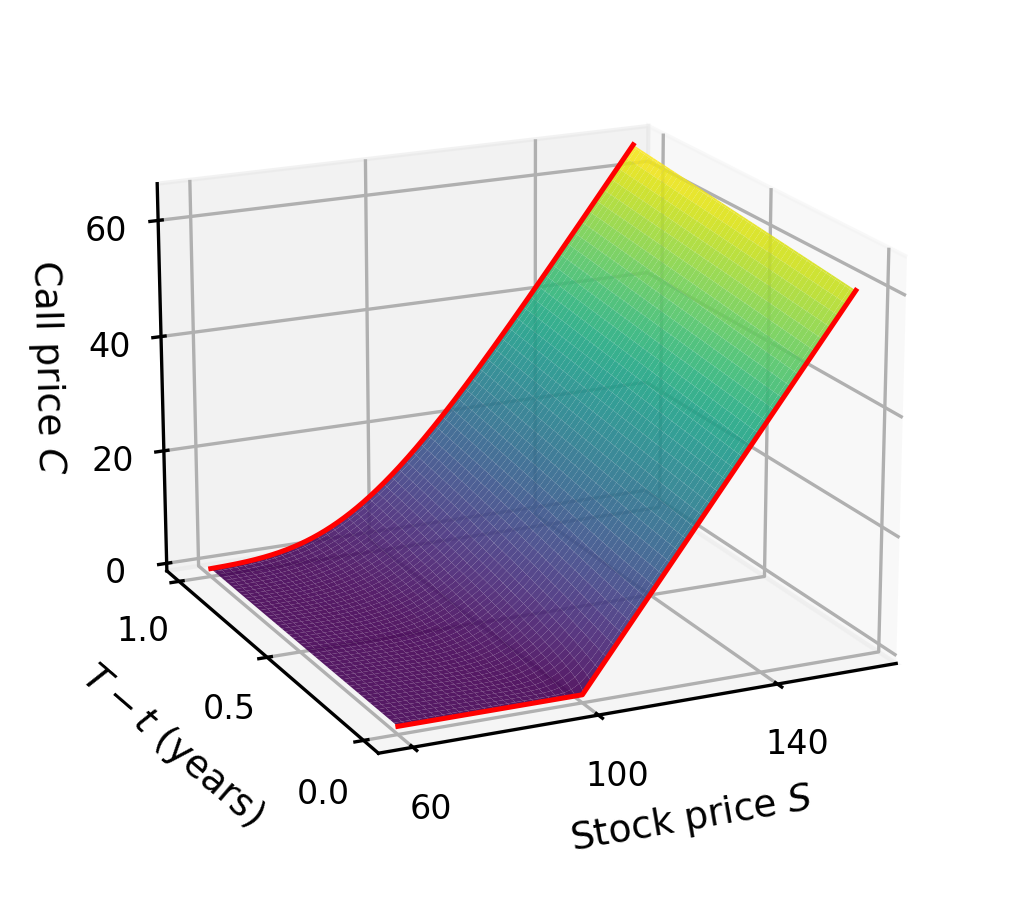
\includegraphics[width=\columnwidth]{Code/figures/exact_solution.png}
\caption{Black-Scholes solution bla bla ( kom tilbake når tallene er riktig)}
\label{fig:exact_solution}
\end{figure}


\begin{figure}[htbp]
\centering
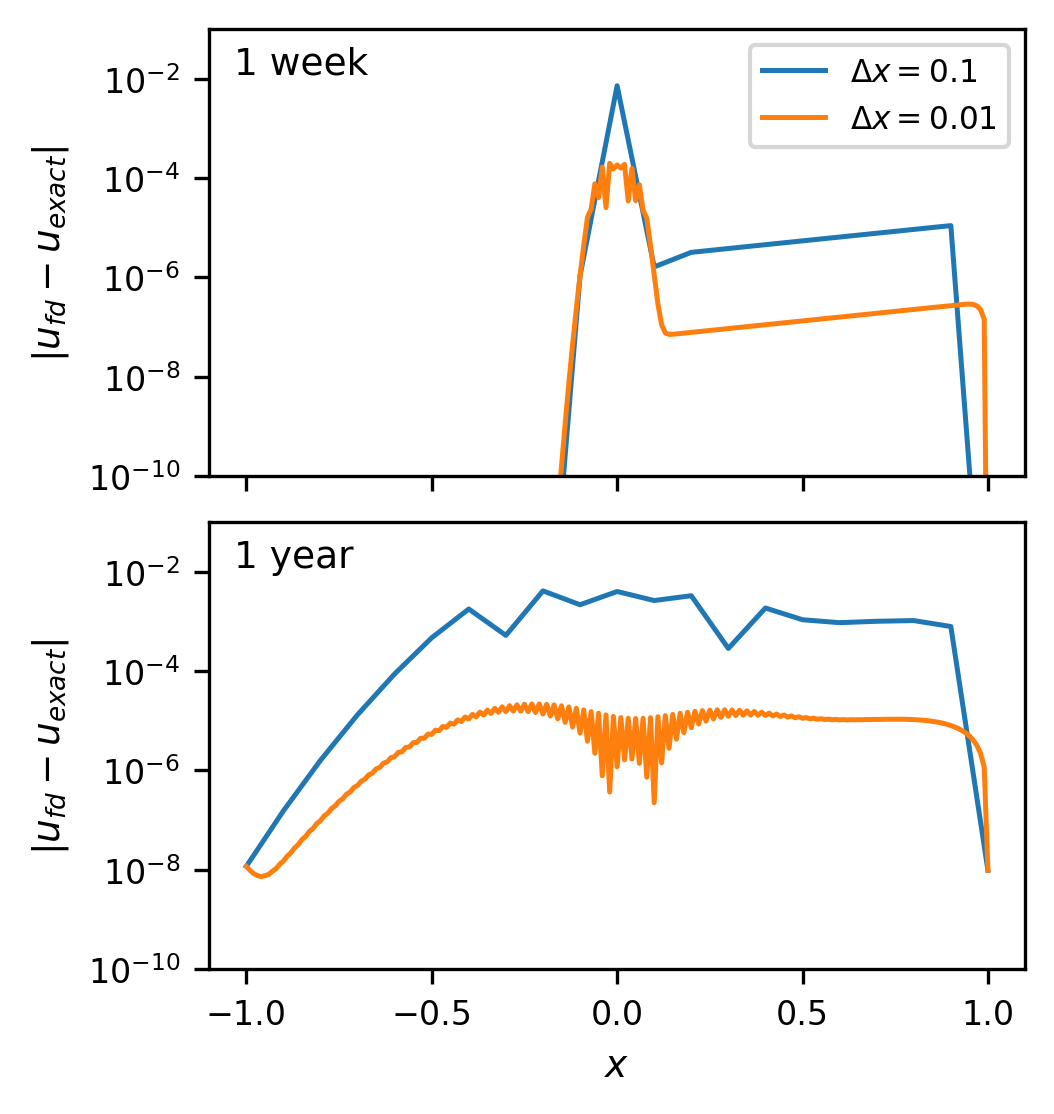
\includegraphics[width=\columnwidth]{Code/figures/fd_profiles.png}
\caption{Feilen skjemaet gjør på BSM}
\label{fig:fd_profiles}
\end{figure}
    %\subsection{The scheme against neural networks}


1. Et kontrollert eksperiment (den viktigste).
Nøyaktig som du sier: ved å ta knekken ut av nettets oppgave skiller dere to mulige feilkilder:

er det knekken som gjør nettet dårlig?
eller er nettet dårlig til opsjonsproblemet generelt?



In Figure~\ref{fig:kink_decomp} our main takeaway is that a kink-free g does not change the scope of the project, just the form. From pointy to smooth is exactly what tanh-network can learn. The figure show why the naive net is going to fail. 

Our naive g is essentially the payoff diagram in the top (black dashed line). 

\begin{figure}[htbp]
\centering
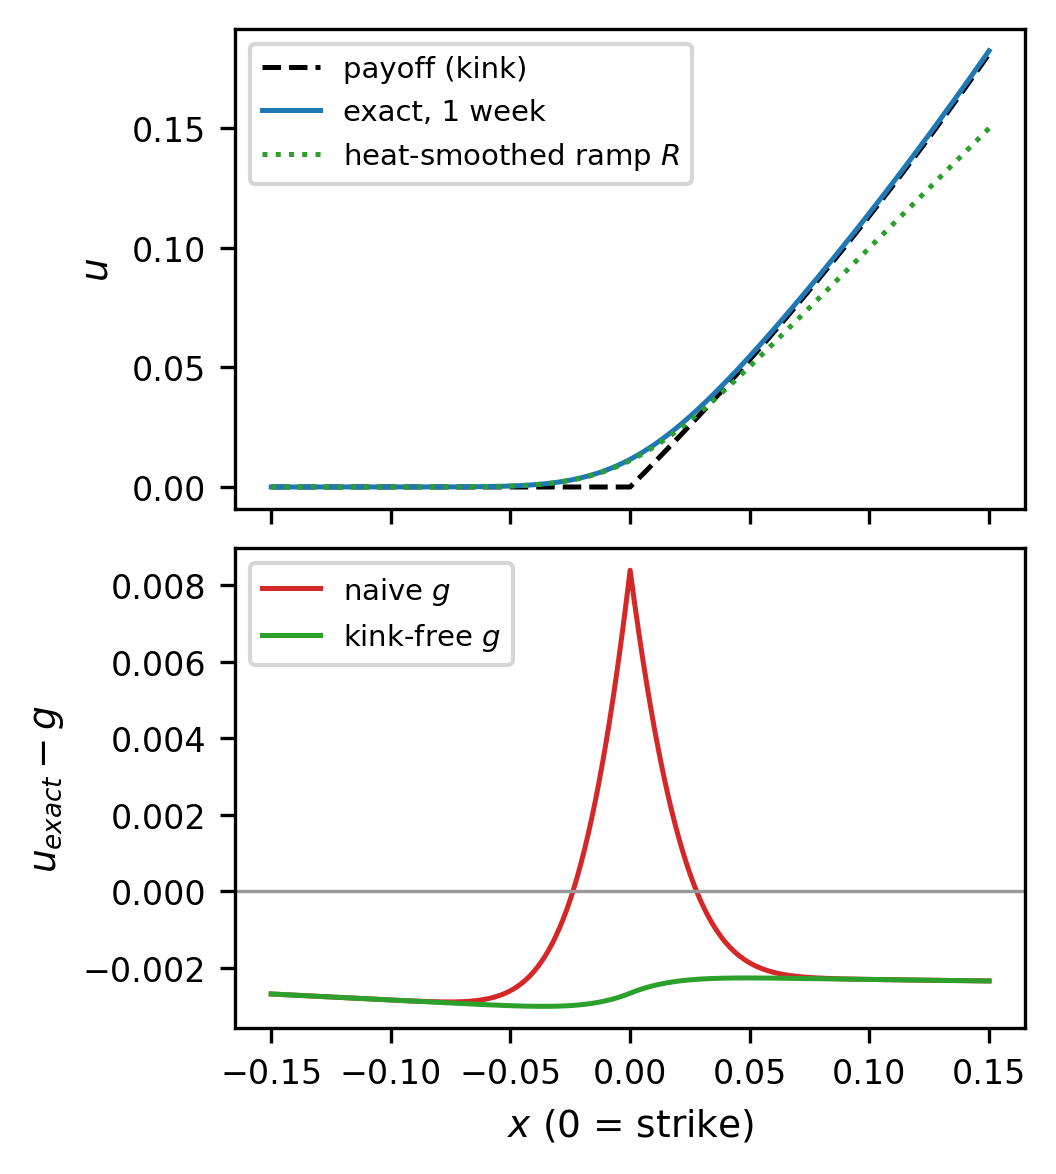
\includegraphics[width=\columnwidth]{Code/figures/kink_decomposition.png}
\caption{\textbf{Top panel:} The solution by 1 week,. \textbf{Bottom panel:} $u_{exact} - g$. For a naive g}
\label{fig:kink_decomp}
\end{figure}

    

    %\input{Sections/RnD3}
    
\section{Conclusion}\label{sec:conclusion}
    %\input{Sections/conclusion}


\bibliography{references}

%TC:ignore
\appendix
\section*{Appendix}
\section{Additional derivations}
    %HUSKELISTE: 

- fikse ledgends, aksetittel, (Figurtittel?), skrifttørrelse.

\section{Declaration of AI use}
    %\subsection{AI tools used}


    %\subsection{Text writing and editing}

    %\subsection{Code generation and assistance}


%TC:endignore

\end{document}

